\section{Data Pipeline: Taasika to UniTime}
\label{sec:pipeline}

\subsection{The source system}

Taasika is the scheduling database already in use at the institution. The project mentor provided a
SQL dump of it, two versions of which are kept in the repository
(\texttt{taasika2-foss-26jan26.sql} and \texttt{taasika3.sql}). The dump stores the data as a series
of numbered \emph{snapshots}, each a complete picture of the departmental schedule at a point in
time. Figure~\ref{fig:taasikaschema} shows the Taasika schema. The corresponding UniTime diagram
is in the repository as \texttt{unitime-schema.png}; reproduced at page size its several hundred
tables are not legible, so it is omitted here. The pipeline is a translation between the two.

\begin{figure}[H]
\centering
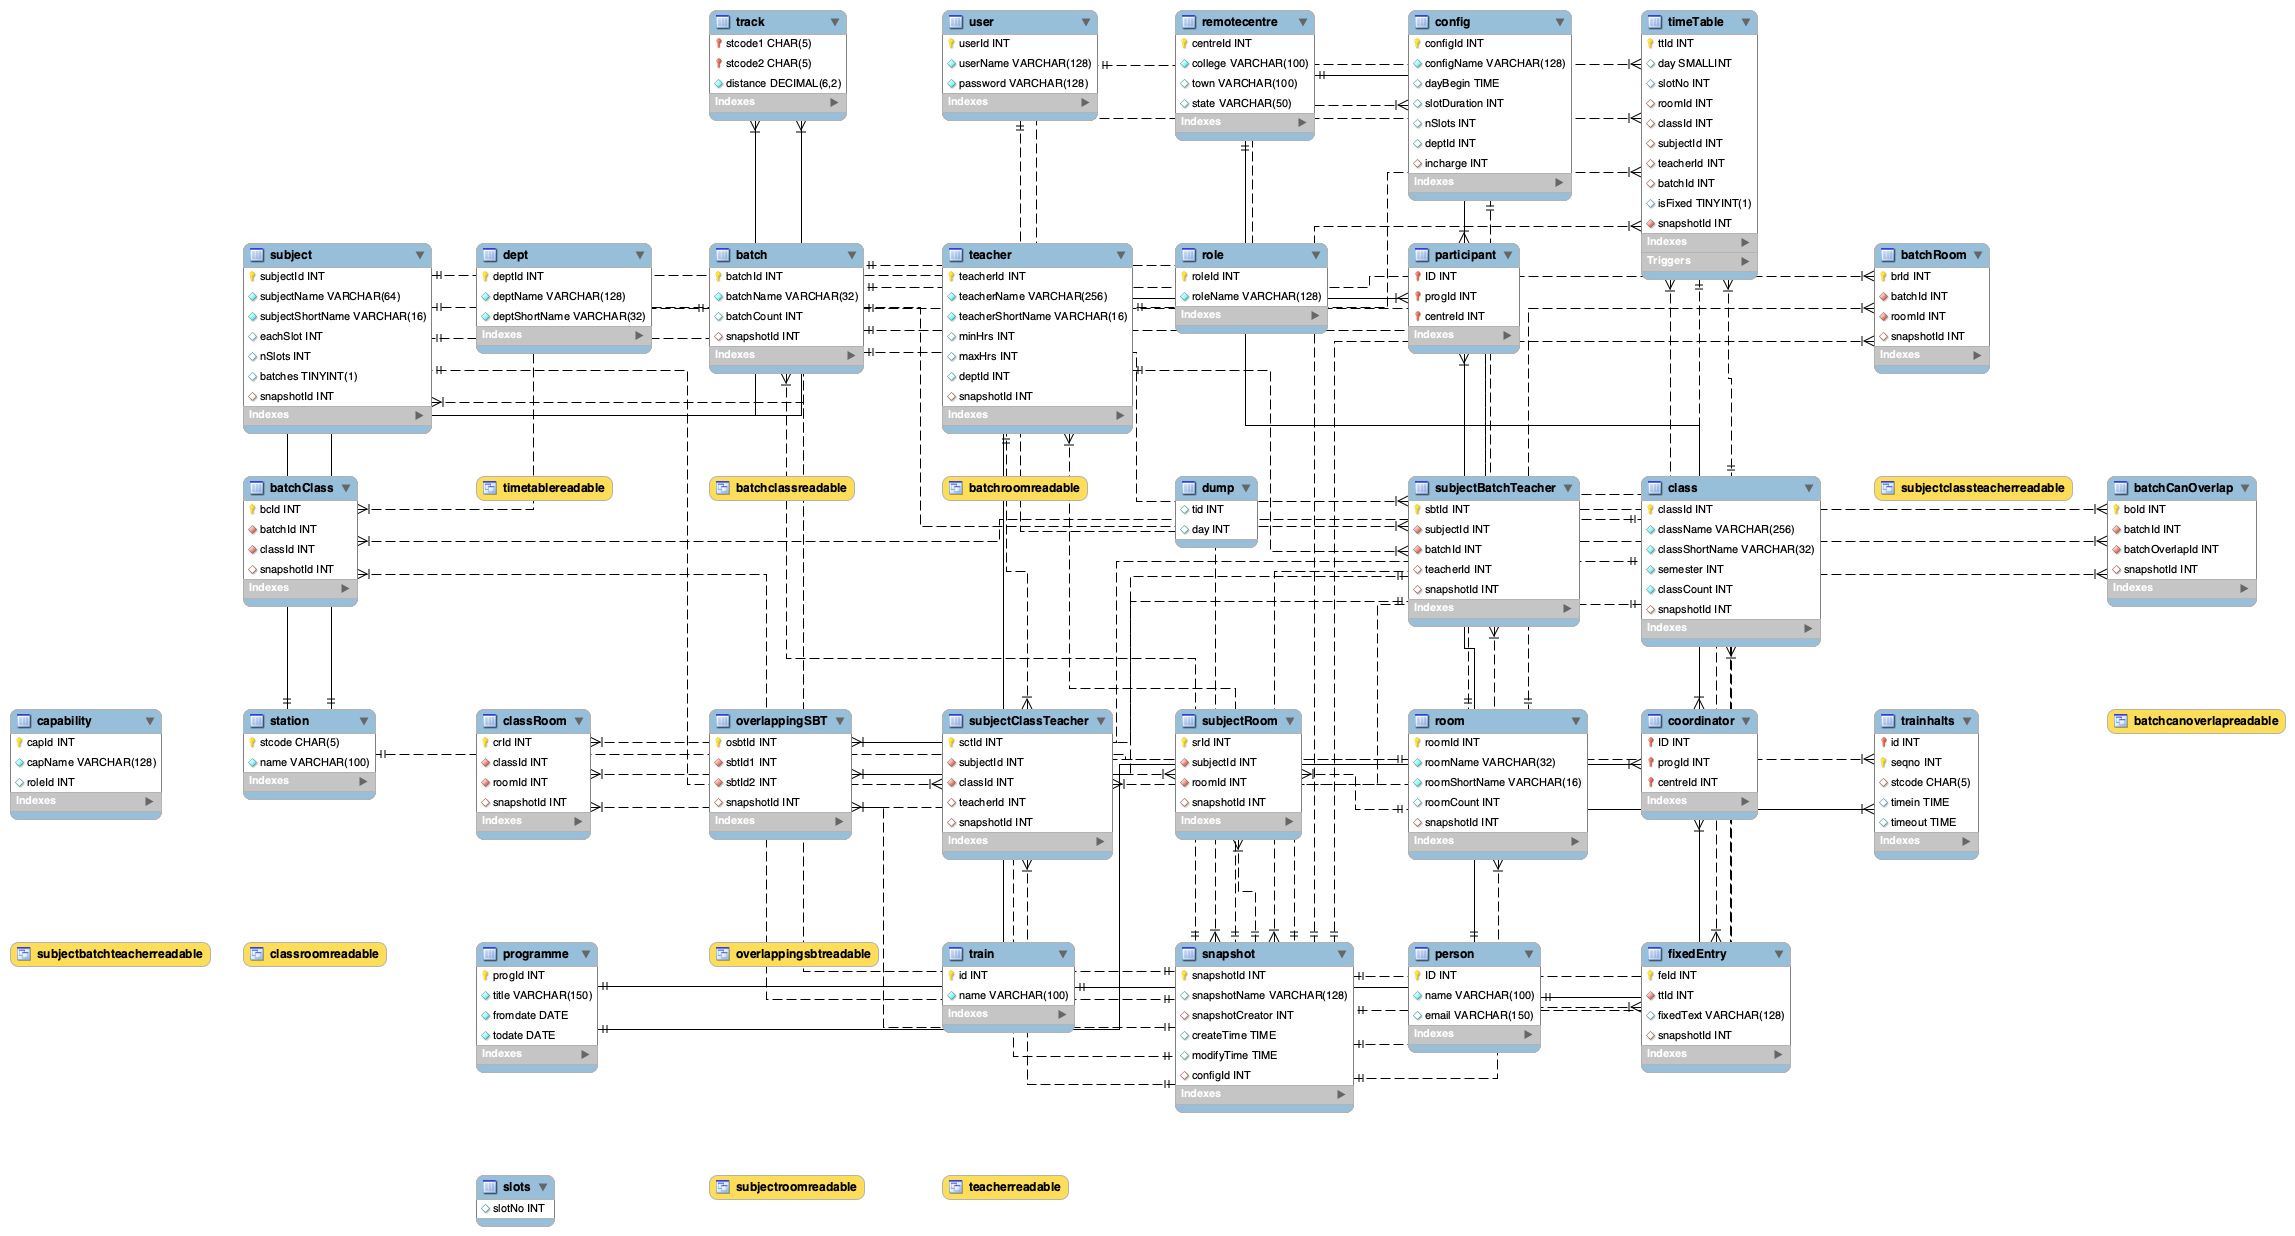
\includegraphics[width=0.62\textwidth]{figures/taasika-schema.png}
\caption{Schema of the Taasika scheduling database, the source of the pipeline.}
\label{fig:taasikaschema}
\end{figure}

A deliberate design decision was to parse the SQL dump textually rather than restore it into a
MySQL server. The loader (\texttt{scripts/taasika\_loader.py}) reads the dump and exposes each table
as a list of Python dictionaries filtered to a chosen snapshot. The pipeline therefore has no
database dependency, runs on any machine with Python, and treats the dump as an immutable input.

\subsection{Pipeline structure}

Figure~\ref{fig:pipeline} shows the complete path from the SQL dump to a scored timetable. Eight
generator modules run in dependency order, three validators check the result, and an archive step
produces the ZIP file that UniTime's Data Exchange page accepts.

\begin{figure}[H]
\centering
\begin{tikzpicture}[
  node distance=5mm and 7mm,
  src/.style={draw,rounded corners=2pt,fill=gray!14,align=center,font=\scriptsize,minimum height=7mm},
  gen/.style={draw,rounded corners=2pt,fill=coepblue!8,align=center,font=\scriptsize,minimum height=7mm},
  xml/.style={draw,fill=coepblue!18,align=center,font=\scriptsize,minimum height=7mm},
  val/.style={draw,rounded corners=2pt,fill=green!10,align=center,font=\scriptsize,minimum height=7mm},
  ut/.style={draw,rounded corners=2pt,fill=orange!14,align=center,font=\scriptsize,minimum height=7mm},
  ev/.style={draw,rounded corners=2pt,fill=red!8,align=center,font=\scriptsize,minimum height=7mm},
  ar/.style={-{Stealth[length=1.8mm]},gray!70}
]
\node[src] (sql) {\texttt{taasika3.sql}\\{\tiny snapshot 242}};
\node[src, right=of sql] (load) {\texttt{taasika\_loader}\\{\tiny textual SQL parse}};
\node[gen, right=of load, text width=30mm] (gens) {8 generators\\{\tiny session, academic, buildings,\\staff, catalog, offerings,\\preferences, students}};
\node[xml, right=of gens, text width=20mm] (xmls) {16 XML files\\{\tiny \texttt{1sessionSetup}\\$\dots$\\\texttt{16studentenrollments}}};

\node[val, below=9mm of gens, text width=34mm] (vals) {validators\\{\tiny \texttt{validate\_xmls},
\texttt{validate\_course\_offering}, \texttt{verify\_time\_patterns}}};
\node[ut, below=9mm of xmls, text width=20mm] (zip) {\texttt{0gen\_all.zip}\\{\tiny flat archive}};

\node[ut, below=9mm of vals, text width=34mm] (ut) {UniTime Data Exchange\\{\tiny import 1\,$\rightarrow$\,16, then solve}};
\node[ev, below=9mm of zip, text width=20mm] (out) {CSV / solver XML\\{\tiny exported solution}};
\node[ev, left=of ut, text width=22mm] (kpi) {\texttt{eval\_timetable\_kpis}\\{\tiny KPI report}};

\draw[ar] (sql) -- (load);
\draw[ar] (load) -- (gens);
\draw[ar] (gens) -- (xmls);
\draw[ar] (xmls) -- (zip);
\draw[ar] (gens) -- (vals);
\draw[ar] (vals) -- (ut);
\draw[ar] (zip) -- (out);
\draw[ar] (ut) -- (out);
\draw[ar] (out) -- (kpi);
\draw[ar] (kpi.north) -- ++(0,6mm) -| node[pos=0.25,above,font=\tiny]{refine} (gens.south west);
\end{tikzpicture}
\caption{The taasika-v3 pipeline. Data flows left to right and top to bottom; the dashed return
path is the refinement loop described in Section~\ref{sec:evaluation}.}
\label{fig:pipeline}
\end{figure}

\subsection{The sixteen imports and why their order matters}

UniTime's Data Exchange interface accepts one document per entity type, and each document
references entities created by an earlier one. The files are numbered so that the import order is
unambiguous; Appendix~\ref{app:imports} lists all sixteen with the dependency that fixes each
position. Three positions are worth highlighting:

\begin{itemize}
  \item \textbf{File 1 is absolute.} \texttt{1sessionSetup.xml} creates the academic session,
    departments, subject areas, solver groups, date patterns and time patterns. Nothing can be
    imported before it exists.
  \item \textbf{File 13 is not optional.} \texttt{13preferences.xml} attaches a time pattern and a
    date pattern to every scheduling subpart. Without it UniTime treats the classes as
    ``arrange hours'' and does not load them into the solver at all, which presents as a solver
    reporting a handful of variables instead of several hundred.
  \item \textbf{Files 14--16 must follow 12.} Student records, course requests and section
    enrolments all reference classes by the identifiers established in
    \texttt{12courseOffering.xml}.
\end{itemize}

Two operational details cost significant time and are recorded here because neither is obvious from
the documentation. First, the term identifier used by the Data Exchange API is the academic term
followed by the year with no separator---\texttt{Spr122026}, not \texttt{2026Spr12}. Second, the
archive must contain the sixteen documents at its \emph{root}; building it with
\texttt{zip -r 0gen\_all.zip 0gen\_all} nests them inside a directory and the import silently fails
to find them. Both the pipeline's own archive step and the standalone
\texttt{scripts/zip\_0gen\_all.py} write entries with a flattened name for this reason.

\subsection{Design decisions}

The Taasika dump does not carry every field UniTime requires, and several structural differences
between the two models had to be resolved by rule rather than by lookup. Table~\ref{tab:decisions}
records the decisions actually implemented in the generators.

\begin{table}[H]
\centering
\caption{Mapping decisions implemented in the generator scripts.}
\label{tab:decisions}
\footnotesize
\begin{tabular}{@{}L{3.5cm}L{11.4cm}@{}}
\toprule
\textbf{Decision} & \textbf{Rule implemented} \\
\midrule
Lecture\,+\,laboratory merging &
  A laboratory or tutorial subject is merged into its lecture partner when its short name is the
  lecture's short name plus one of \texttt{-Lab}, \texttt{Lab}, \texttt{-Tut}, \texttt{Tut} or
  \texttt{-Tutorial}. The merged course becomes one offering with one configuration and two
  subparts, so joint lectures and parallel batches live under a single course. \\
Course credits &
  The Indian engineering convention: one credit per lecture hour and half a credit per laboratory
  hour, so a three-hour lecture paired with a two-hour laboratory yields four credits. Unpaired
  subjects use the lecture-only or laboratory-only half of the same formula, with a floor of one. \\
Class identifiers &
  Human-readable and stable: \texttt{"<area> <courseNbr> <type> <suffix>"}, for example
  \texttt{CS 110 Lab 3}. These identifiers are what files 15 and 16 reference. \\
Building inference &
  Taasika stores room names but not buildings. A heuristic on the room name and short name assigns
  each room to one of six inferred buildings; unavailable laboratories are collected into their own
  pool so that their use remains visible in the KPI report. \\
Instructor position &
  Derived from each teacher's \texttt{minHrs}/\texttt{maxHrs} envelope: at most 6 hours maps to
  professor, at most 12 to associate professor, otherwise assistant professor, with
  $(0,0)$ mapped to adjunct and $(0,24)$ to visitor. \\
Times left unsolved &
  No class carries a \texttt{<time>} element. The existing Taasika timetable rows are deliberately
  not imported as preferences, because the object of the exercise is for UniTime to solve the
  timetable rather than to reproduce the manual one. \\
Rooms as preferences &
  Room associations from Taasika are emitted as preferences, not as pre-assignments, leaving the
  solver free to choose. \\
Student simulation &
  The institution's MIS data was not available, so students are generated from confirmed headcounts
  (Section~\ref{sec:datasets}) with synthetic identifiers of the form \texttt{61yy03aaa}. \\
\bottomrule
\end{tabular}
\end{table}

\subsection{Entry point and validation}

The whole pipeline is driven by one command, which selects the SQL dump and snapshot, runs the
eight generators in order, runs the three validators, and writes the archive only if all three
pass:

\begin{lstlisting}[style=plainlst,language=bash,caption={Regenerating the complete dataset.}]
python scripts/gen_all.py --term Spr12 --sql taasika-db/taasika3.sql --snapshot 242
\end{lstlisting}

The validators check three different properties. \texttt{validate\_xmls.py} confirms that every
generated document is well-formed XML. \texttt{validate\_course\_offering.py} checks the structural
invariants of file 12---that every class belongs to a subpart, every subpart to a configuration,
and every configuration to an offering---before UniTime is given the chance to reject it.
\texttt{verify\_time\_patterns.py} re-derives each subject's weekly minutes from the Taasika
snapshot and confirms that the time pattern emitted in file 13 matches, which catches the class of
error where a course silently becomes unschedulable because its duration has no matching pattern.

A separate script, \texttt{scripts/zip\_0gen\_all.py}, re-targets an existing dataset to a new term
and rebuilds the archive without regenerating from SQL. This exists because a fresh UniTime
academic session is often the fastest way to recover from a bad import, and creating one requires
only that the term attribute change.
